\documentclass[10pt,mathserif]{beamer}

\usepackage{graphicx,amsmath,amssymb,tikz,psfrag,subfigure,bm}

\input defs.tex

%% formatting

\mode<presentation>
{
\usetheme{default}
}
\setbeamertemplate{navigation symbols}{}
\usecolortheme[rgb={0,0,0}]{structure}
\setbeamertemplate{itemize subitem}{--}
\setbeamertemplate{frametitle} {
	\begin{center}
	  {\large\bf \insertframetitle}
	\end{center}
}

\AtBeginSection[] 
{ 
	\begin{frame}<beamer> 
		\frametitle{Outline} 
		\tableofcontents[currentsection,currentsubsection] 
	\end{frame} 
} 

%% begin presentation

\title{\large \bfseries Adaptive basis function models}

\author{Jiali Lin\\[3ex]
Virginia Tech}

\date{\today}

\begin{document}

\frame{
\thispagestyle{empty}
\titlepage
}

\section{Introduction}
\begin{frame}{Introduction}
\begin{itemize}
    \item Consider kernel methods to create non-linear models for regression and classification.
    \item The prediction takes the form $f(\bm{x}) = \bm{w}^T \phi(\bm{x})$,
    where $\phi(\bm{x})$ is kernel.
    \item Coming up with a good kernel function is quite difficult.
    \item \textbf{Goal:} dispense with kernels altogether, and try to learn useful features $\phi(\bm{x})$ directly from the input data.
    \item \textbf{Adaptive basis function model (ABM)} has the form
    \begin{equation*}
        f(\bm{x}) = w_0 + \sum_{m=1}^M w_m\phi_m(\bm{x})
    \end{equation*}
\end{itemize}
\end{frame}

\section{Classification and regression trees (CART)}
\begin{frame}{Basics}
Consider the tree in Figure.
\begin{figure}[h]
\centering
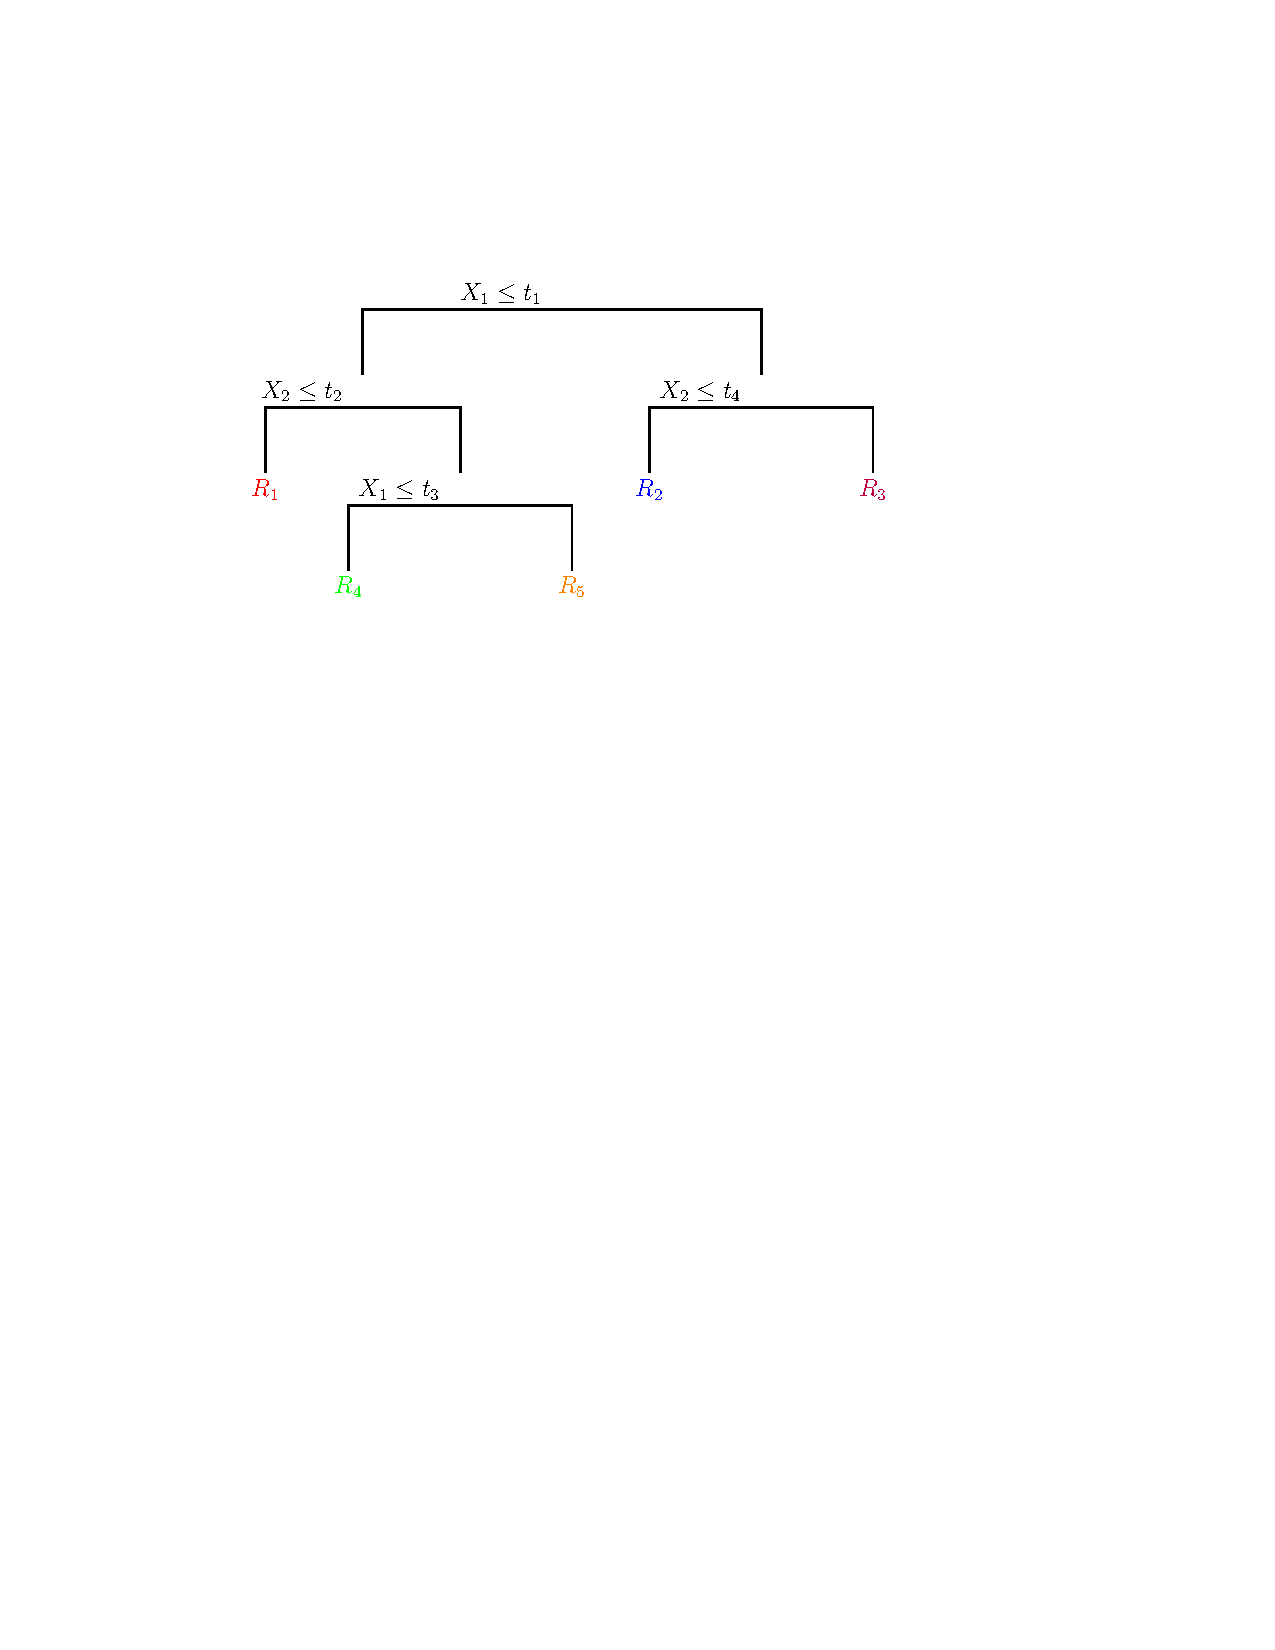
\includegraphics[width=0.4\textwidth]{regtree}
\caption{The first node asks if $x_1$ is less than some threshold $t_1$. If yes, we then ask if $x_2$ is less than some other threshold $t_2$. If yes, we are in the bottom left quadrant of space, $R_1$. If no, we ask if $x_1$ is less than $t_3$. And so on. The result of these axis parallel splits is to partition 2d space into 5 regions.}
\end{figure}

We can write the model in the following form
\begin{equation*}
    f(\bm{x}) = E[y|\bm{x}] = \sum_{m=1}^M w_m \mathbb{I}(\bm{x} \in R_m) = \sum_{m=1}^M w_m \phi(\bm{x}; \bm{v}_m)
\end{equation*}

where $R_m$ is the $m$'th region, $w_m$ is the mean response in this region, and $\bm{v}_m$ encodes the choice of variable to split on.
\end{frame}

\begin{frame}{Growing a tree}
\begin{itemize}
    \item Finding the optimal partitioning of the data is NP-complete.
    \item Methods to compute a locally optimal MLE: \textbf{CART}, \textbf{C4.5} and \textbf{ID3}.
    \item  The split function chooses the best feature, and the best value for that feature
    \begin{equation*}
        (j^*, t^*) = \min_{j\in\{1,\ldots,D\}}\min_{t\in\mathcal{T}_j}\text{cost}({\bm{x}_i, y_i: x_{ij} \leq t}) + \text{cost}({\bm{x}_i, y_i: x_{ij}> t})
    \end{equation*}
    where $\mathcal{T}_j$ is set of possible thresholds for feature $j$.
    \item Split function checks if a node is worth splitting can use several stopping heuristics.
    \item Cost measure depends on whether our goal is regression or classification.
\end{itemize}
\end{frame}

\begin{frame}{Cost}
\begin{itemize}
    \item \textbf{Regression cost}
    \begin{equation*}
        \text{cost}(\mathcal{D}) =  \sum_{i\in \mathcal{D}}(y_i - \bar{y})^2
    \end{equation*}
    where $\bar{y} = \frac{1}{|\mathcal{D}|}\sum_{i\in \mathcal{D}}y_i$.
    \item \textbf{Classification cost:}
    First, we fit a multinoulli model to the data in the leaf satisfying the test $X_j < t$ by estimating
        \begin{equation*}
            \hat{\pi_c} = \frac{1}{|D|}\sum_{i\in D}\mathbb{I}(y_i = c)
        \end{equation*}
    Several ways to measure the quality of a split:
    \begin{itemize}
        \item \textbf Misclassification rate.
        \item Entropy, or deviance.
        \item Information gain.
        \item Gini index.
    \end{itemize}
\end{itemize}
\end{frame}

\begin{frame}{Example}
\begin{figure}[h]
\centering
\subfigure[]{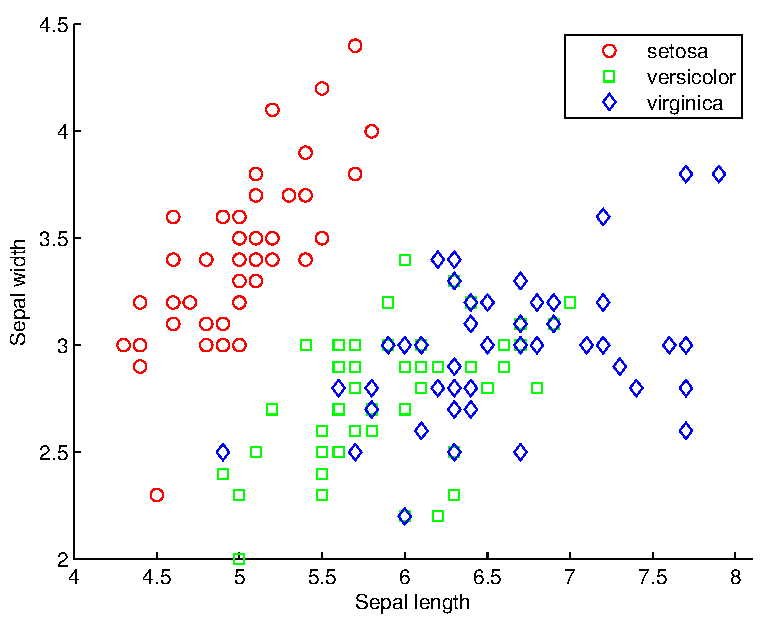
\includegraphics[width=20mm]{dtreeIrisData}}
\subfigure[]{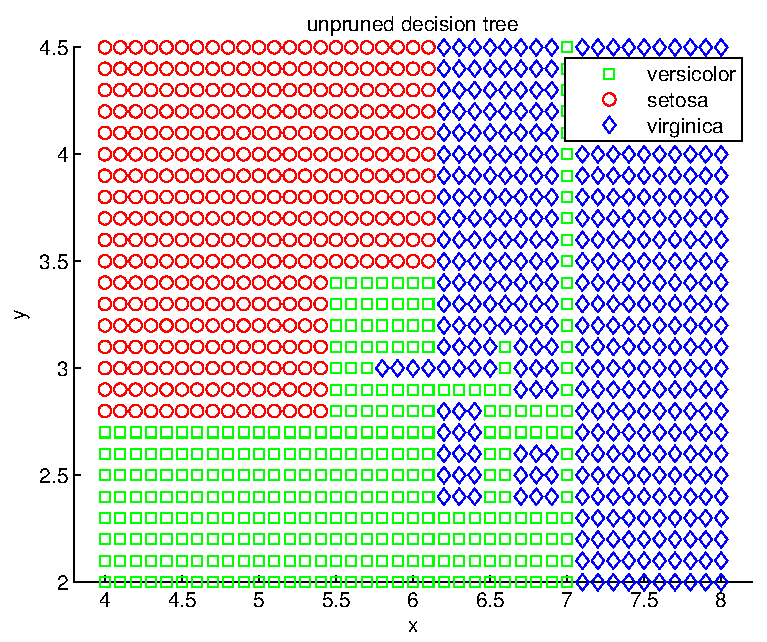
\includegraphics[width=20mm]{dtreeDboundaryUnpruned}}
\caption{(a) Iris data. We only show the first two features, sepal length and sepal width, and ignore petal length and petal width. (b) Decision boundaries induced by the decision tree in Figure 2(a).}
\end{figure}

\begin{figure}[h]
\centering
\subfigure[]{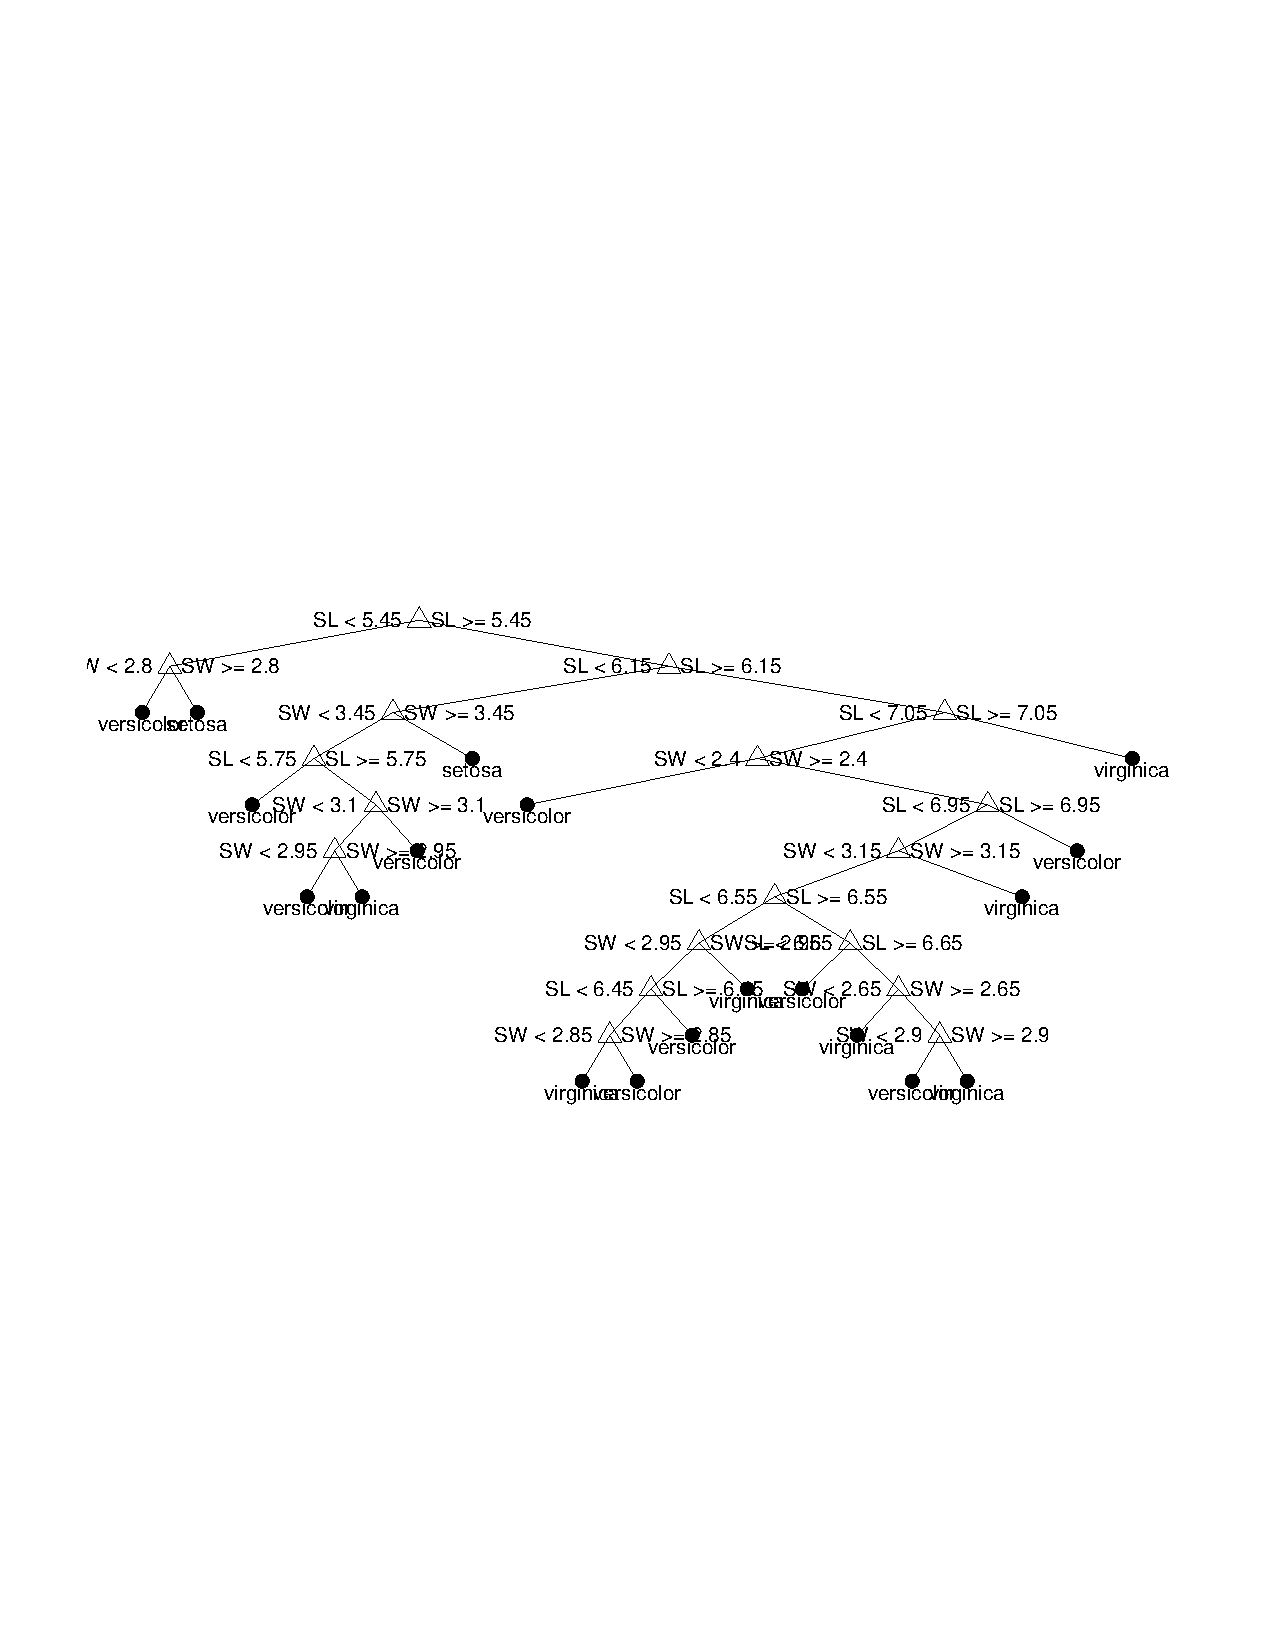
\includegraphics[width=20mm]{dtreeUnprunedTree}}
\subfigure[]{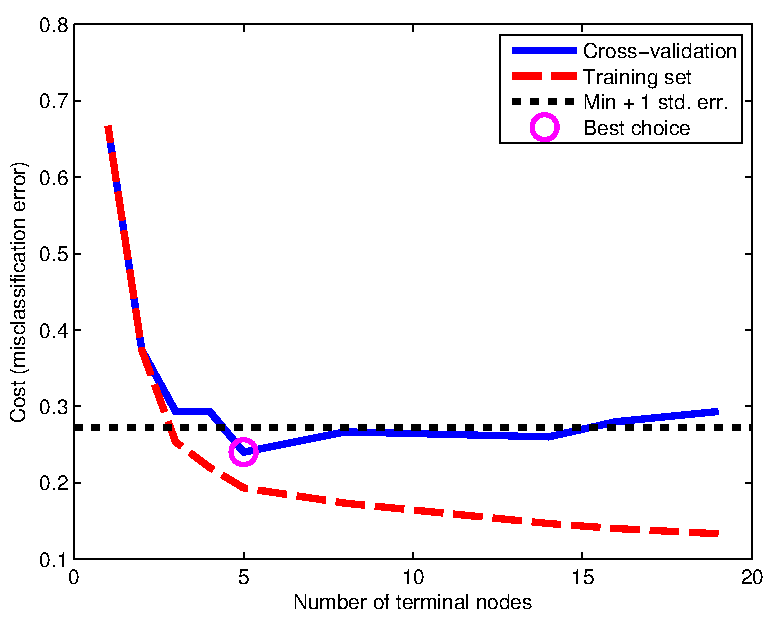
\includegraphics[width=20mm]{dtreeErrorVsDepth}}
\caption{(a) Unpruned decision tree for Iris data. (b) Plot of misclassification error rate vs depth of tree. Figure generated by \texttt{dtreeDemoIris}.}
\end{figure}
\end{frame}

\begin{frame}{Pruning a tree}
\begin{itemize}
    \item Motivation: prevent overfitting. 
    \item Idea: grow a ``full" tree, and then to perform \textbf{pruning}.
    \item How far to prune back? Evaluate the cross-validated error on each subtree.
    \item Biggest \textbf{cons}: unstable! outlier can leads to high variance trees.
\end{itemize}
\end{frame}

\begin{frame}{Random forests}
\begin{itemize}
    \item Reduce the variance of an estimate:  average together many estimates (say $M$ trees)
    \begin{equation*}
        f(\bm{x}) =  \sum_{m=1}^M \frac{1}{M}f_m(\bm{x})
    \end{equation*}
    where $f_m$ is the $m$'th tree (This is called \textbf{bagging}).
    \item Problems: can result in highly correlated predictors.
    \item \textbf{Random forests} decorrelates the base learners by learning trees based on a randomly chosen subset of input variables and datasets.
\end{itemize}
\end{frame}

\section{Boosting}
\begin{frame}{Introduction}
\begin{itemize}
    \item \textbf{Boosting:} a greedy algorithm for fitting ABMs, where the $\phi_m$ are generated by an algorithm called a \textbf{weak learner} or a \textbf{base learner}.
    \item Idea: applying the weak learner sequentially to weighted versions of the data.
    \item More weight is given to examples that were misclassified by earlier rounds.
    \item \textbf{Goal:} solve the optimization problem
    \begin{equation*}
        \min_f \sum_{i=1}^N L(y_i, f(\bm{x}_i))
    \end{equation*}
\end{itemize}

\begin{table}[h!]
\centering
\resizebox{\columnwidth}{!}{%
\begin{tabular}{ c c c c c}
 Name & Loss & Derivative & Minimizers $f^*$ & Algorithm\\ 
 \hline
 Squared error & $\frac{1}{2}(y_i - f(\bm{x}_i))^2$ & $y_i - f(\bm{x}_i)$ & $E[Y|\bm{x}_i]$ & L2Boosting \\  
 Absolute error & $|y_i - f(\bm{x}_i)|$ & $\text{sign}(y_i - f(\bm{x}_i))$ & $\text{median}(y|\bm{x}_i)$ & Gradient boosting \\
 Exponential loss & $\exp(-\tilde{y_i}f(\bm{x}_i))$ & $-\tilde{y_i}\exp(-\tilde{y_i}f(\bm{x}_i))$ & $\frac{1}{2}\log\frac{\pi_i}{1-\pi_i}$ & AdaBoost \\
 Logloss & $\log(1+e^{-\tilde{y_i}f_i})$ & $y_i - \pi_i$ & $\frac{1}{2}\log\frac{\pi_i}{1-\pi_i}$ & LogitBoost \\ [1ex] 
\end{tabular}%
}
\caption{Some commonly used loss functions. Assume $\tilde{y}_i \in \{-1,+1\}$, $y_i \in \{0,1\}$ and $\pi_i = \text{sigm}(2f(\bm{x}_i))$. For regression problems, we assume $y_i\in \mathbb{R}$.}
\label{table:1}
\end{table}
\end{frame}

\begin{frame}{Generalized additive models}
\begin{itemize}
    \item Finding the optimal $f$ may be hard, we shall tackle it sequentially. 
    \item We initialise by defining
    \begin{equation*}
        f_0(\bm{x}) = \min_{\bm{\gamma}} \sum_{i=1}^N L(y_i,f(\bm{x}_i;\bm{\gamma}))
    \end{equation*}
    \item Then at iteration $m$, we compute 
    \begin{equation*}
        (\beta_m, \bm{\gamma}_m) = \min_{\beta, \bm{\gamma}} \sum_{i=1}^N L(y_i,f_{m-1}(\bm{x}_i) + \beta\phi(\bm{x}_i; \bm{\gamma}))
    \end{equation*}
    \item Then, we set 
    \begin{equation*}
        f_m(\bm{x})= f_{m-1}(\bm{x}) + \beta_m\phi(\bm{x};\bm{\gamma}_m)
    \end{equation*}
    \item \textbf{Key:} do not go back and adjust earlier parameters. This is called \textbf{forward stagewise additive modeling}.
    \item In practice,  we do ``partial updates" 
    \begin{equation*}
        f_m(\bm{x})= f_{m-1}(\bm{x}) + \nu\beta_m\phi(\bm{x};\bm{\gamma}_m)
    \end{equation*}
    where $0 < \nu \leq 1$ is a step-size parameter (called \textbf{shrinkage}).
\end{itemize}
\end{frame}

\begin{frame}{L2boosting}
\begin{itemize}
    \item Suppose we used squared error loss. Then at step $m$ the loss
    \begin{equation*}
        L(y_i,f_{m-1}(\bm{x}_i) + \beta\phi(\bm{x}_i;\bm{\gamma})) = (r_{im} - \phi(\bm{x}_i;\bm{\gamma}))^2
    \end{equation*}
    where $r_{im} = y_i - f_{m-1}(\bm{x}_i)$ is the current residual, and we have set $\beta = 1$.
    \item We can find the new basis function by using the weak learner to predict $\bm{r}_m$.
\end{itemize}
\end{frame}

\begin{frame}{AdaBoost}
\begin{itemize}
    \item Consider a binary classification problem with exponential loss. At step $m$ we have to minimize
    \begin{equation*}
        L_m(\phi) = \sum_{i=1}^N \exp[-\tilde{y}_i(f_{m-1}(\bm{x}) + \beta\phi(\bm{x}_i))] = \sum_{i=1}^N w_{i,m}\exp(-\beta\tilde{y}_i\phi(\bm{x}_i))
    \end{equation*}
     where $w_{i,m} = \exp(-\tilde{y}_i(f_{m-1}(\bm{x})))$ is a weight applied to datacase $i$.
    \item Rewrite this objective as follows
    \begin{equation*}
        \begin{split}
            L_m & = e^{-\beta} \sum_{\tilde{y}_i = \phi(\bm{x}_i)} w_{i,m} + e^\beta \sum_{\tilde{y}_i \neq \phi(\bm{x}_i)} w_{i,m} \\
            & = (e^{\beta} - e^{-\beta} )\sum_{i=1}^N w_{i,m} \mathbb{I}(\tilde{y}_i \neq \phi(\bm{x}_i)) + e^{-\beta}\sum_{i=1}^N w_{i,m}
        \end{split}
    \end{equation*}
\end{itemize}
\end{frame}

\begin{frame}{AdaBoost (cont'd)}
\begin{itemize}
    \item Consequently the optimal function to add is
    \begin{equation*}
        \phi_m  = \argmin_{\phi} w_{i,m} \mathbb{I}(\tilde{y}_i \neq \phi(\bm{x}_i))
    \end{equation*}
    \item After finding $\phi_m$, subsitute $\phi_m$ into $L_m$
    \begin{equation*}
        \beta_m = \frac{1}{2}\log\frac{1-\text{err}_m}{\text{err}_m}
    \end{equation*}
    where 
    \begin{equation*}
        \text{err}_m = \frac{\sum_{i=1}^N w_i \mathbb{}(\tilde{y}_i \neq \phi_m(\bm{x}_i))}{\sum_{i=1}^N w_{i,m}}
    \end{equation*}
    \item The overall updates becomes 
    \begin{equation*}
        f_m(\bm{x})= f_{m-1}(\bm{x}) + \beta_m\phi_m(\bm{x})
    \end{equation*}
\end{itemize}
\end{frame}

\begin{frame}{AdaBoost (cont'd)}
The weights at the next iteration become
\begin{equation*}
    \begin{split}
        w_{i,m+1} & = w_{i,m}e^{-\beta_m \tilde{y}_i\phi_m(\bm{x}_i)}\\
        & = w_{i,m}e^{\beta_m(2\mathbb{I}(\tilde{y}_i\neq\phi_m(\bm{x}_i))-1)}\\
        & = w_{i,m}e^{2\beta_m\mathbb{I}(\tilde{y}_i\neq\phi_m(\bm{x}_i))}e^{-\beta_m}
    \end{split}
\end{equation*}
    
where we exploited that $-\tilde{y}_i\phi_m(\bm{x}_i) = -1$ if $\tilde{y}_i = \phi_m(\bm{x}_i)$ and $-\tilde{y}_i\phi_m(\bm{x}_i) = +1$ otherwise. Since $e^{-\beta_m}$ will cancel out in the normalization step, we can drop it. 

\noindent\rule[-5pt]{\textwidth}{0.4pt}
{\footnotesize
\begin{tabbing}
    {\bf given} $w_i= 1/N$. \\*[\smallskipamount]
    {\bf for} $m=1:M$ {\bf do}\\
    \qquad \= 1.\ Fit a classifier $\phi_m(\bm{x})$ to the training set using weights $w$. \\
    \> 2.\ Compute $\text{err}_m = \frac{\sum_{i=1}^N w_i I(\tilde{y}_i \neq \phi_m(\bm{x}_i))}{\sum_{i=1}^N w_{i,m}}$. \\
    \> 3.\ Compute $\alpha_m = \log\frac{1-\text{err}_m}{\text{err}_m}$. \\
    \> 4.\ Set $w_i\leftarrow w_i\exp\left[\alpha_m\mathbb{I}(\tilde{y}_i\neq\phi_m(\bm{x}_i))\right]$. \\*[\smallskipamount]
    {\bf return} $f(\bm{x})=\text{sgn}\left[\sum_{m=1}^M\alpha_m\phi_m(\bm{x}))\right]$.
\end{tabbing}}
\noindent\rule[10pt]{\textwidth}{0.4pt}
\end{frame}

\begin{frame}{Why does boosting work so well?}
\begin{figure}[h]
\centering
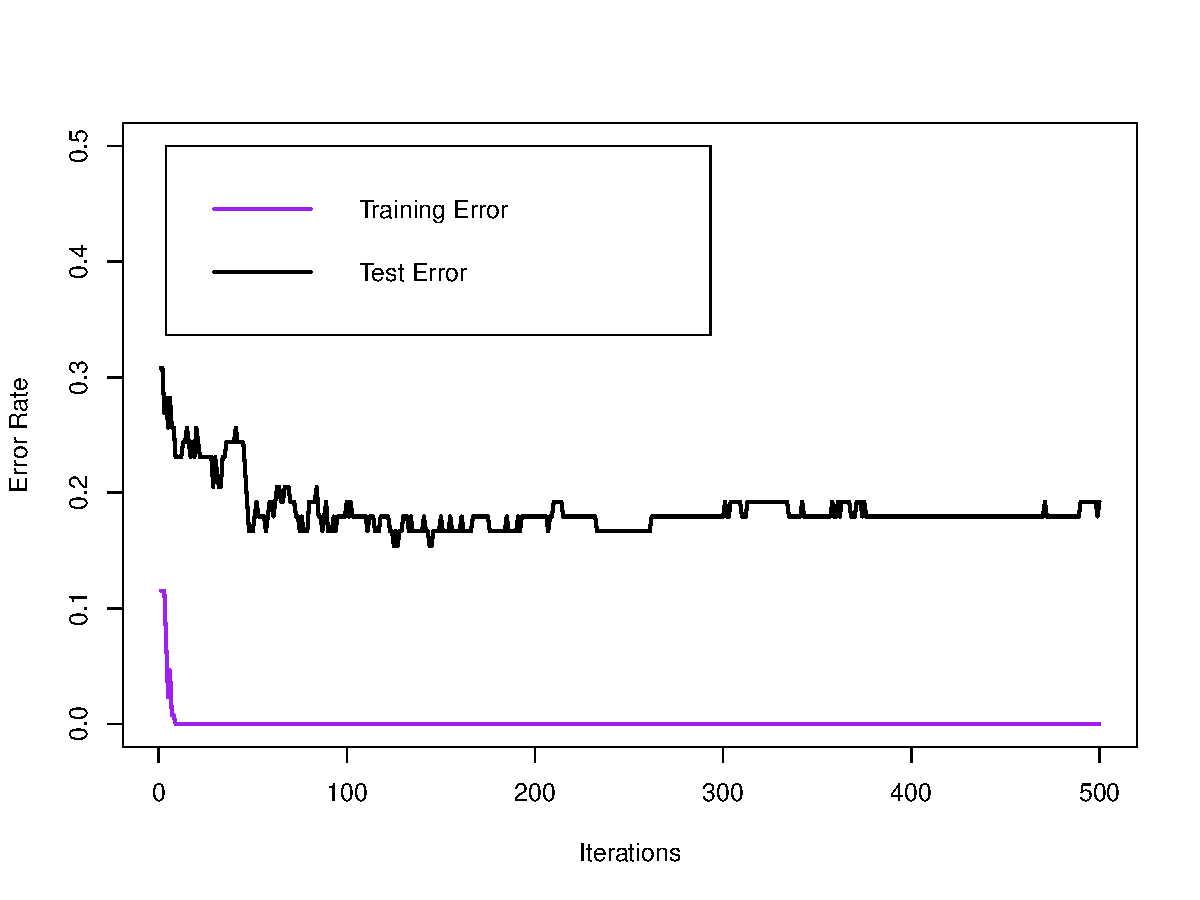
\includegraphics[width=0.5\textwidth]{AdaboostDemo}
\caption{Illustration of AdaBoost. AdaBoost is very slow to overfit. Figure generated by \texttt{AdaboostDemo}.}
\end{figure}
\begin{itemize}
    \item Can be viewed as ``$\ell_1$ regularization": use $\ell_1$ regularization to select a subset, $\phi(\bm{x}) = [\phi_1(\bm{x}),\ldots,\phi_K(\bm{x})]$.
    \item It can be proved that AdaBoost maximizes the margin on the training data.
\end{itemize}    
\end{frame}

\begin{frame}{LogitBoost}
\begin{itemize}
    \item Exponential loss  puts a lot of weight on misclassified examples.
    \item Therefore, exponential loss is sensitive to outliers (mislabeled examples).
    \item Cannot recover probability estimates from $f(\bm{x})$, $\exp(-\tilde{y_i}f(\bm{x}_i))$ ss not the logarithm of any pmf for binary variables $\tilde{y}_i \in \{-1,+1\}$.
\end{itemize}
\begin{figure}[h]
\centering
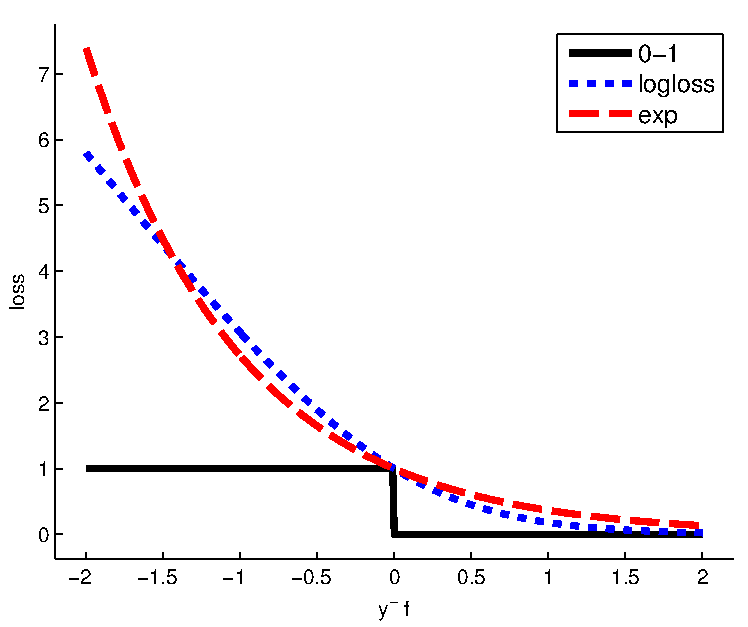
\includegraphics[width=0.4\textwidth]{expLoss}
\caption{ Illustration of various loss functions for binary classification. Figure generated by \texttt{hingeLossPlot}.}
\end{figure}
\end{frame}

\begin{frame}{LogitBoost (cont'd)}
\begin{itemize}
    \item \textbf{Logloss} only punishes mistakes linearly.
    \item It means we will be able to extract probabilities from the final learned function, by \begin{equation*}
        p(y = 1|\bm{x}) = \frac{e^{f(\bm{x})}}{e^{-f(\bm{x})} + e^{f(\bm{x})}} = \frac{1}{e^{-2f(\bm{x})} + 1}
    \end{equation*}
    \item The goal is to minimze the expected log-loss, given by
    \begin{equation*}
        L_m(\phi) = \sum_{i=1}^N \log \left[1 + \exp(-2\tilde{y}_i(f_{m-1}(\bm{x}) + \phi(\bm{x}_i)))\right]
    \end{equation*}
\end{itemize}

\noindent\rule[-5pt]{\textwidth}{0.4pt}
{\footnotesize
\begin{tabbing}
    {\bf given} $w_i= 1/N, \pi_i =1/2$. \\*[\smallskipamount]
    {\bf for} $m=1:M$ {\bf do}\\
    \qquad \= 1.\ Compute the working response $z_i =\frac{y^* - \pi}{\pi_i(1 - \pi_i)}$. \\
    \> 2.\ Compute the weights $w_i = \pi(1 - \pi)$. \\
    \> 3.\ Compute $\phi_m = \argmin_\phi \sum_{i=1}^N w_i(z_i-\phi(\bm{x}_i))^2$. \\
    \> 4.\ Update $f(\bm{x}) \leftarrow f(\bm{x}) + \frac{1}{2}\phi_m(\bm{x})$. \\
    \> 5.\ Compute $\pi = 1/(e^{-2f(\bm{x}_i)} + 1)$. \\*[\smallskipamount]
    {\bf return} $f(\bm{x})=\text{sgn}\left[\sum_{m=1}^M\phi_m(\bm{x}))\right]$.
\end{tabbing}}
\noindent\rule[10pt]{\textwidth}{0.4pt}
\end{frame}

\begin{frame}{Boosting as functional gradient descent}
\begin{itemize}
    \item \textbf{Gradient boosting}: imagine minimizing
    \begin{equation*}
        \hat{\bm{f}} = \min_{\bm{f}} L(\bm{f})
    \end{equation*}
    where $\bm{f} = (f(\bm{x}_1 ),\ldots, f(\bm{x}_N))$ are the ``parameters". 
    \item At step $m$ let $\bm{g}_m$ be the gradient of $L(\bm{f})$ evaluated at $\bm{f} = \bm{f}_{m-1}$:
    \begin{equation*}
        g_{im}  = [\frac{\partial L(y_i, f(\bm{x}_i))}{\partial f(\bm{x}_i)}]_{f = f_{m-1}}
    \end{equation*}
    \item Then make the update
    \begin{equation*}
        \bm{f}_m = \bm{f}_{m-1} - \rho_m \bm{g}_m
    \end{equation*}
    where $\rho_m$ is the step length, chosen by
    \begin{equation*}
        \rho_m = \min_\rho L(\bm{f}_{m-1} - \rho \bm{g}_m)
    \end{equation*}
\end{itemize}
\end{frame}

\begin{frame}{Boosting as functional gradient descent (cont'd)}
\begin{itemize}
    \item We only optimizes $f$, but do not learn a function that can generalize.
    \item Modify the algorithm by fitting a weak learner to approximate the negative gradient signal
    \begin{equation*}
        \bm{\gamma}_m = \min_{\bm{\gamma}} \sum_{i=1}^N (-g_{im} - \phi(\bm{x}_i,\bm{\gamma}))^2
    \end{equation*}
\end{itemize}

\noindent\rule[-5pt]{\textwidth}{0.4pt}
{\footnotesize
\begin{tabbing}
    {\bf Initialize} $f_0(\bm{x} ) = \min_{\bm{\gamma}} \sum_{i=1}^N L(y_i, f(\bm{x}_i))$. \\*[\smallskipamount]
    {\bf for} $m=1:M$ {\bf do}\\
    \qquad \= 1.\ Compute the gradient residual using $r_{im}  = - [\frac{\partial L(y_i, f(\bm{x}_i))}{\partial f(\bm{x}_i)}]_{f(\bm{x}_i)= f_{m-1}(\bm{x}_i)}$. \\
    \> 2.\ Compute the weights $w_i = \pi(1 - \pi)$. \\
    \> 3.\ Use the weak learner to compute $\bm{\gamma}_m$ which minimizes $\sum_{i=1}^N (r_{im} - \phi(\bm{x}_i,\bm{\gamma}))^2$. \\
    \> 4.\ Update $f_m(\bm{x}) = f_{m-1}(\bm{x})  + \nu\phi(\bm{x};\bm{\gamma}_m)$. \\*[\smallskipamount]
    {\bf return} $f(\bm{x})=f_M(\bm{x})$.
\end{tabbing}}
\noindent\rule[10pt]{\textwidth}{0.4pt}    
\end{frame}

\section{Ensemble learning}
\begin{frame}{Stacking}
\begin{itemize}
    \item \textbf{Ensemble learning:} learning a weighted combination of base models
    \begin{equation*}
        f(y|\bm{x},\bm{\pi})=   \sum_{m\in M}w_m f_m(y|\bm{x})
    \end{equation*}
    \item Estimate the weights
    \begin{equation*}
        \hat{\bm{w}} = \min_{\bm{w}} \sum_{i=1}^N L(y_i,\sum_{m=1}^M w_m f_m(\bm{x}))
    \end{equation*}
    \item However, this will result in overfitting, with $w_m$ being large for the most complex model.
    \item \textbf{Solution:} use the LOOCV estimate
    \begin{equation*}
        \hat{\bm{w}} = \min_{\bm{w}} \sum_{i=1}^N L(y_i,\sum_{m=1}^M w_m f_m^{-1}(\bm{x})).
    \end{equation*}
    where $f_m^{-1}(\bm{x})$ is the predictor obtained by training on data excluding $(\bm{x}_i, y_i)$
    \item This is known as \textbf{stacking}, which stands for ``stacked generalization". 
\end{itemize}
\end{frame}

\end{document}
